\documentclass[fontset=windows]{article}
\usepackage[margin=1in]{geometry}%设置边距,符合Word设定
\usepackage{ctex}
\usepackage{amsmath, xparse}
\usepackage{amssymb}
\usepackage{setspace}
\usepackage{lipsum}
\usepackage{graphicx}%插入图片
\graphicspath{{Figures/}}%文章所用图片在当前目录下的 Figures目录
\usepackage{hyperref} % 对目录生成链接,注:该宏包可能与其他宏包冲突,故放在所有引用的宏包之后
\hypersetup{
    colorlinks        = true,  % 将链接文字带颜色
	bookmarksopen     = true, % 展开书签
	bookmarksnumbered = true, % 书签带章节编号
	pdftitle          = 关于曲线的弯曲性质的研究, % 标题
	pdfauthor         = DarkSharpness, % 作者
    citecolor         = black,
    linkcolor         = red,
    urlcolor          = blue}
\bibliographystyle{plain}% 参考文献引用格式
\newcommand{\upcite}[1]{\textsuperscript{\cite{#1}}}

\renewcommand{\contentsname}{\centerline{Contents}} %经过设置word格式后,将目录标题居中
% Keywords command
\providecommand{\keywords}[1]
{
  \textbf{\text{Keywords: }} #1
}


\title{\heiti\zihao{2} 关于曲线的弯曲性质的研究}
\author{DarkSharpness}
\date{2022.12.31}

\begin{document}
	\maketitle
	% \thispagestyle{empty}

% 摘要
\begin{abstract} 
    本文从曲线的定义入手,借助正则曲线的弧长参数表示,重新定义了曲线的切向等基本参数;从低维入手逐步推导了曲线的曲率、法向、挠率和副法向等基本参量,并指明了其背后的物理意义以及其与曲线弯曲程度的关系;最后本文将推导出表征任意维度的曲线弯曲程度的所有基本参量。
\end{abstract}


\keywords{正则曲线 , 弧长参数 , 曲率 , 挠率 , 高阶曲率 , 曲线的弯曲程度.}

\tableofcontents

\section*{引言}

平面曲线在生活中处处可见,各种屏幕上显示出来的图形的轮廓就是由二维的平面曲线构成,而各种文字也是由平面曲线构成。而对于平面曲线,我们可以很直观的感觉的不同曲线在不同地方弯曲程度不同。例如下图中的一条直线和一个圆,我们很明显能感知到圆的弯曲程度要大于直线。

\begin{figure}[htb]
	\centering
	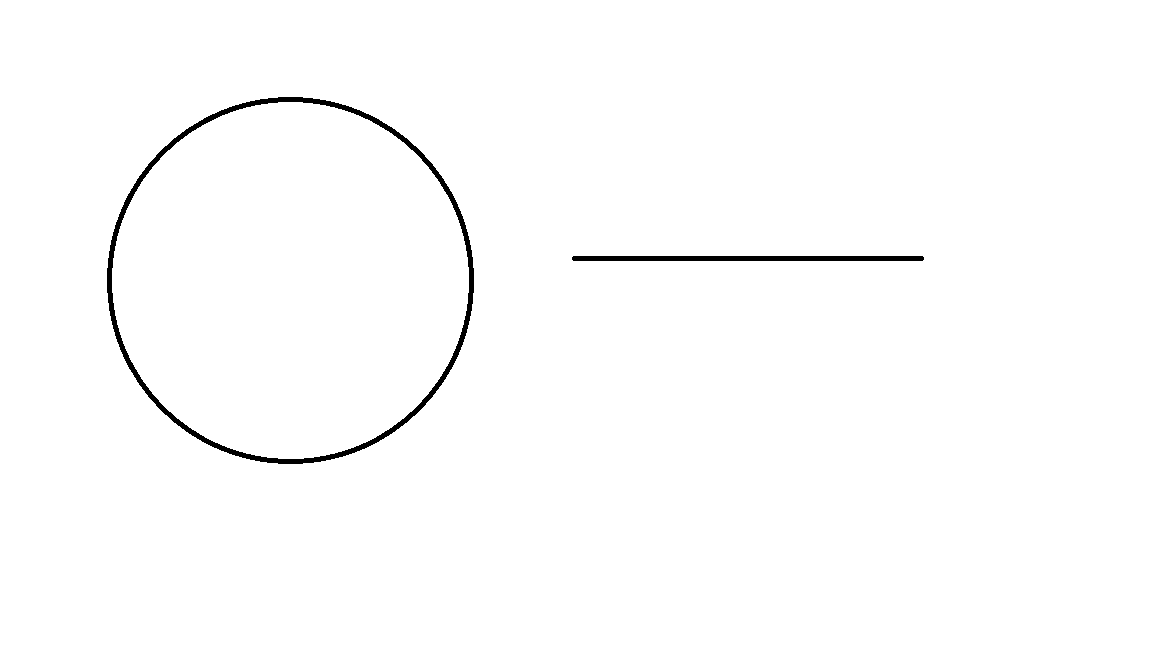
\includegraphics[scale=0.3]{1.png}
	\caption{}
\end{figure}

然而,这样的对于“弯曲程度”的感知只是一种直觉上的感知,是基于比较且不能量化的。对于给定参数的一个平面曲线,我们应该发展出数学的工具来给出一个点附近弯曲程度的严格定义。而到了高维度,甚至是超过了我们所生活的三维空间更高维度,我们的直觉就完全失效了。这就更加需要我们发展出一套数学理论来解决这样的问题。

事实上,这样的理论工具在生活中也大有用处。它可以和物理学、工程学等结合,进而用于解决实际生活的一些问题。

因此,本文将对刻画曲线弯曲程度的所有参数进行研究,探索其解析形式。

\section{一般曲线的表示}

\subsection{弧长参数}

在数学上,一条曲线的定义为:设 ${\displaystyle I=[a,b]}\ I=[a,b]$ 为一实数区间,即实数集的非空子集,那么曲线 $c$ 就是一个连续函数 $c : I → X$ 的映像,其中 $X$ 为一个拓扑空间。\upcite{ref1}

因此,对于 $\mathbb{R}^n$ 的任意一条曲线,我们都可以把其写成每一个维度的分量关于参数 $t$ 的形式,记作 $x_i = x_i(t)$ 。因此,曲线的位矢可写作展开形式 $\vec{r} = (x_1(t),x_2(t),...,x_n(t))$ ,其中 $t \in [a,b]$ 。

然而,这样的的表示是不完美的,其存在一个与曲线本身无直接关联的参数 $t$ 。例如,对于任意 $t'$ 和单调增函数 $f$ 满足 $f(t') \in [a,b] \ (t\in[c,d])$ ,$t$ 和 $t'$ 存在一一映射的关系。因此, $\vec{r} = (x_1(t),x_2(t),...,x_n(t)) = (x_1(f(t')),x_2(f(t')),...,x_n(f(t'))) = (x_1'(t'),x_2'(t'),...,x_n'(t'))$。可以看出,曲线的表示依赖于参数 $t$ 的选取,将 $t$ 替换为 $t'$ 之后,曲线的表示发生改变。这显然不是一个很本质的表示。

事实上,我们可以考虑下参数 $t$ 的现实意义,在一条曲线相同位置固定 $d\vec{r}$ 的情况下,选择不同的参数, $dt$ 也会不同。若把 $t$ 当作为时间,$\vec{r}$ 当作位移,那么不同的 $t$ 则对应了我们在曲线上移动的速度  $\frac{d\vec{r}}{dt}$ 不同。

为了解决这一问题,我们引入新的一个参数 $s$,定义 $ds = \sqrt{dx_1^2+dx_2^2+...+dx_n^2}$ ,$ s= \int{ds} + C $。

为了简化讨论,我们将讨论范围局限于 \textbf{正则曲线\upcite{ref2}},即满足 $\vec{r}$ 对于 $t$ 处处可微的曲线。此时,将 $\vec{r(t)}$ 可写作 $\vec{r(s)}$。由复合函数求导公式, $\frac{d\vec{r}}{ds} = \frac{d\vec{r}/dt}{ds/dt}$ 。而注意到 $|d\vec{r}| = \sqrt{dx_1^2+dx_2^2+...+dx_n^2}$,因此 $|\frac{d\vec{r}}{ds}| = 1$。该参数与曲线本身密切相关,用前面的现实意义去分析,$s$ 就可以理解为固定速度为1的在曲线上移动。

我们将上述参数定义为\textbf{弧长参数},其是一个只与曲线本身相关的曲线的参数表示,其中曲线需要满足正则曲线的性质。

\subsection{切线}

在最开始发展微分理论的时候,导数就是用来求出函数在一个点的切线方向的工具。在平面直角坐标系中,函数一点的切线的一个方向向量为 $(1,\frac{dy}{dx})$ 。而对于任意的可弧长参数化的曲线 $\vec{x} = \vec{x}(s) $ ,我们可以回到切线的定义去求出切线方向。我们设切线这条直线的参数形式为 $\vec{y} = \vec{y}(s)$ ,在 $ s = s_0 $ 处相切,因此 $\vec{y}(s_0) = \vec{x}(s_0)$ ,且在 $s_0$ 附近,两条曲线要尽可能地接近。令 $\delta{s} =s -s_0$ ,则:

$$
\begin{aligned}
|\vec{y}(s) - \vec{x}(s)| 
&= \sqrt{\sum_{i=1}^{n}{(y_i(s) - x_i(s)) ^ 2}} \\
&= \sqrt{\sum_{i=1}^{n}{(\frac{dy}{ds}-\frac{dx}{ds})^2 \cdot\delta{s}^2} + o({(δs)^2})} \\
&= |\frac{d\vec{y}}{ds} - \frac{d\vec{x}}{ds}| \cdot \delta{s} +o(\delta{s})
\end{aligned}
$$

不难看出,当切线满足 $\frac{d\vec{y}}{ds} = \frac{d\vec{x}}{ds} (s=s_0)$ 时候,在 $s_0$ 附近两者最接近,所以曲线地切线方向地一个方向向量即为 $\frac{d\vec{x}}{ds}$ 。注意到 $|\frac{d\vec{x}}{ds}| = 1$,所以其也是切向的单位向量。记\textbf{单位切向量}为 $\vec{T} = \frac{d\vec{x}}{ds}$ ,满足 $|\vec{T}| = 1$。

\section{二维曲线}

为了简单起见,我们先从二维的情况开始讨论。

\subsection{二维曲线的法向量与曲率}

二维曲线在一个平面内,除了切向量,其还存在恰好一个方向向量与切向量相切,记这个方向为\textbf{法向}。此时,由于 $|\vec{T}| = 1$ ,因此 $\vec{T} \cdot \vec{T} = 1$ 。左右对 $s$ 求导,$\frac{d\vec{T}}{ds} \cdot \vec{T} = 0$ 。因此可以得出,$\frac{d\vec{T}}{ds} \perp \vec{T}$ ,其沿法向。我们记\textbf{单位法向量} $\vec{N} = \frac{\frac{d\vec{T}}{ds}}{|\frac{d\vec{T}}{ds}|} $ 。

而曲线的曲率被定义为曲线转动的快慢,即在一个点附近切向转过角度与偏离位移大小的比值的极限。对于二维的曲线,因为在弧长参数下 $\vec{T}$的模长保持不变,其装过的角度 $\delta \theta = \frac{|\delta{\vec{T}}|}{|T|} = |\delta{\vec{T}}|  $ ,如下图所示。

\begin{figure}[htb]
	\centering
	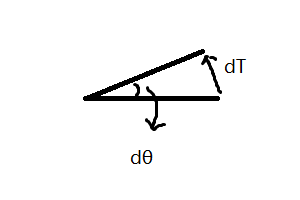
\includegraphics[scale=1]{2.png}
	\caption{}
\end{figure}

因此,记\textbf{曲率}为 $\kappa$ ,由定义,$\kappa = \lim_{\delta s \rightarrow 0}{\frac{\delta \theta}{\delta s}} = \lim_{\delta s \rightarrow 0}{\frac{|\delta {\vec{T}}|}{\delta s}}\cdot{\frac1{|\vec{T}|}} = |\frac{d\vec T}{ds}|$ ,所以由单位法向量 $\vec{N}$ 的定义,$\frac{d\vec T}{ds} = \kappa \vec{N}$ 。 在一般情况下,我们还用记曲率半径 $\rho = \frac1{\kappa}$ 。对于一个特殊的曲线:圆,该曲率半径就等于圆的半径。

总结一下,我们大致可以得到如下的定义式:

$$
\begin{aligned}
    \vec{T} &= \frac{d\vec{r}}{ds} \\
    \kappa  &= |\frac{d\vec{T}}{ds}| \\
    \vec{N} &= \frac{1}{\kappa} \frac{d\vec{T}}{ds} \\
            &= \frac{1}{\kappa} \frac{d^2{\vec{r}}}{ds}
\end{aligned}
$$

% \subsection{切向量、法向量与曲率的其他性质}

% 由上,在二维弧长参数 $\vec{r} = \vec{r}(s)$ 下 ,我们已经定义了如下三个量:

% $$
% \begin{aligned}
% \vec{T} &= \frac{d\vec{r}}{ds} \\
% \kappa  &= |\frac{d\vec{T}}{ds}| \\
% \vec{N} &= \frac{1}{\kappa} \cdot \frac{d\vec{T}}{ds} \\
% \end{aligned}
% $$

% 而这些量之间还存在一些内在的联系。由 $|\vec{T}| = 1$,即 $\vec{T}\cdot\vec{T} = 1 $ ,对两边求二阶导,$\frac{d^2\vec{T}}{ds^2} \cdot T + (\frac{d\vec{T}}{ds})^2 = 0 $ 此时由定义以及 $|\vec{N}| = 1$ ,有 $\frac{d^2\vec{T}}{ds^2} \cdot \vec{T} = -\kappa^2$。记为(1)式。

% 类似的,因为 $|\vec{N}| = 1$ 即 $\vec{N}\cdot\vec{N} = 1$,我们对两边对 $s$ 求导 $\vec{N}\cdot \frac{d\vec{N}}{ds} = 0$ ,所以可知 $\vec{N} \perp \frac{d\vec{N}}{ds}$。又因为已经证过 $\vec{T} \perp \frac{d\vec{T}}{ds} = \kappa\cdot{\vec{N}}$ ,所以 $\frac{d\vec{N}}{ds} $ 与 $\vec{T}$ 共线。再带入 ${\vec N} $ 的定义,以及(1)式,可知 $\frac{d{\vec{N}}}{ds} = -\kappa \vec{T}$

% 因此,我们可以总结出下面几个常用的式子。

% $$
% \begin{aligned}
% \vec{T} &= \frac{d\vec{r}}{ds} \\
% \vec{N} &= \frac{1}{\kappa} \cdot \frac{d^2\vec{r}}{ds^2} \\
% \\
% \frac{d\vec{T}}{ds} &= {\kappa} \cdot {\vec{N}} \\
% \frac{d\vec{N}}{ds} &= -{\kappa} \cdot {\vec{T}} \\
% \\
% \frac{d^2\vec{T}}{ds^2} &= - \kappa ^ 2 \cdot \vec{T} \\
% \end{aligned}
% $$

\subsection{法向量与切向量的现实意义}

事实上,回到最初的含有 $t$ 的参数表示形式,我们只需将每一个 $ds$ 换为 $\frac{ds}{dt} \cdot dt$ 即可。而此时,$\frac{ds}{dt}$ 对于的是现实世界中的运动速度,而 $t$ 对应的是时间。将上述式子整理化简,我们可以得到:

$$
\begin{aligned}
\frac{ds}{dt}\cdot\vec{T} &= \frac{d\vec{r}}{dt} \\
\kappa \cdot (\frac{ds}{dt}) ^ 2 \cdot \vec{N} + \frac{d^2s}{dt^2}\cdot\vec{T} &= \frac{d^2\vec{r}}{dt^2}  \\
\end{aligned}
$$

而在物理中,两个式子的右边分别对应的是速度矢量和加速度矢量。左边的 $\frac{ds}{dt}$ 为速度大小,$\frac{d^2s}{dt^2}$ 为速度大小的变化率。可以看出,质点在曲线上运动的时候,除了切线方向速度大小改变带来切向加速度,由曲率还会带来一项法向的加速度,这便是人们常说的向心加速度。而通过二维曲线切向量法向量相关的知识,我们便能很容易地研究二维曲线上的质点运动问题,处理这类问题有很多其他的数学工具,这里就不展开说明了。

\section{三维曲线}

\subsection{三维曲线的法向和曲率}

对于三维曲线,其切线方向的单位向量依然可以由 $T = \frac{d\vec{r}}{ds}$ 得出。而对于三维的曲线,与其垂直的方向构成了一个平面。因此,我们不能像二维那样将法向定义为与切向垂直的方向,因为这样的方向有无数个。然而,我们依然可以从法线的另外一个性质“切向量变化的方向”入手,来定义法向量。类似二维曲线,通过切向量转过的角度的大小与通过距离的比值,我们依然可以定义\textbf{曲率} $\kappa = \lim_{\delta s \rightarrow 0}{\frac{δθ}{δs}} = \lim_{\delta s \rightarrow 0}{\frac{|\delta {\vec{T}}|}{\delta s}}\cdot{\frac1{|\vec{T}|}} = |\frac{d\vec T}{ds}|$ 。而我们将切向量变化的方向定义为 \textbf{法向},则可以得到与二维情况下相同的形式 $\vec{N} = \frac1{\kappa}\cdot\frac{d\vec{T}}{ds}$。

\subsection{三维曲线的副法向与挠率}
由上,我们已经可以得到相互正交的两个方向:切向和法向。但在一个三维空间中,任何一组标准正交基应当存在三个互相垂直单位向量。因此,我们可以通过叉乘给出第三个单位向量,记\textbf{副法向的单位向量} $\vec{B} = \vec{T} \times \vec{N}$ 。此时,$\vec{T},\vec{N},\vec{B}$ 构成了该三维空间中的一组标准正交基。

由正交性,$\vec N \cdot \vec T = 0$ 。两边对 $s$ 求导,并带入 $\vec N = \frac1{\kappa} \cdot \frac{d\vec T}{ds} $,可得 $\frac{d\vec N}{ds} \cdot \vec T = -\kappa$ 。记为(1)式。

由于 $|\vec{N}| = 1$ 即 $\vec N \cdot \vec N = 1$ ,两边对 $s$ 求导有 $\vec N\cdot \frac{d\vec N}{ds} = 0$ 可知 $\vec N \perp \frac{d\vec N}{ds}$ 。因此,可在标准正交基框架下设 $\frac{d\vec N}{ds} = \alpha \vec T + \beta \vec B $。记为(2)式。

将(2)带入(1),可知 $\alpha = -\kappa$ 。

而类似(2)式,我们可以设 $\frac{d\vec B}{ds} = \gamma \vec T + \xi \vec N $ ; 类似(1) 式,我们也能写出 $\frac{d\vec B}{ds} \cdot \vec T = -\vec{B} \cdot \frac{d\vec T}{ds} $ 以及 $ \frac{d\vec B}{ds} \cdot \vec N = -\vec{B} \cdot \frac{d\vec N}{ds} $ 。容易求出,$\gamma = 0,\xi = -\beta$。

汇总一下,我们可以得到如下这些式子。

$$
\begin{aligned}
\vec{T} &= \frac{d\vec{r}}{ds}\\
\\
\frac{d\vec T}{ds} &= \kappa \cdot \vec N \\
\frac{d\vec N}{ds} &= -\kappa \cdot \vec T + \beta \cdot \vec B\\
\frac{d\vec B}{ds} &= -\beta \cdot \vec N \\
\end{aligned}
$$

其中,$\vec B$ 是由 $\vec T \times \vec N$ 定义得到,$\beta$ 是一个曲线相关的常数,其大小等于 $|\frac{d\vec N}{ds} + \kappa \cdot \vec T|$,称为\textbf{挠率}。

\subsection{挠率的几何直观}

至今为止,我们只是从理论上推导出了挠率的值,却没有给出其背后的意义。我们对上述最后一个式子取模长,有 $|\beta| = |\frac{d\vec B}{ds}|$。而利用 定义式: $\vec B = \vec T \times \vec N$ ,我们可以得到:$\beta$ 的大小等于副法向量转动的角度的快慢,即法向量切向量构成的平面转动的角度 $\delta \phi$ 与 $ds$ 的比值的极限。

\begin{figure}[htb]
	\centering
	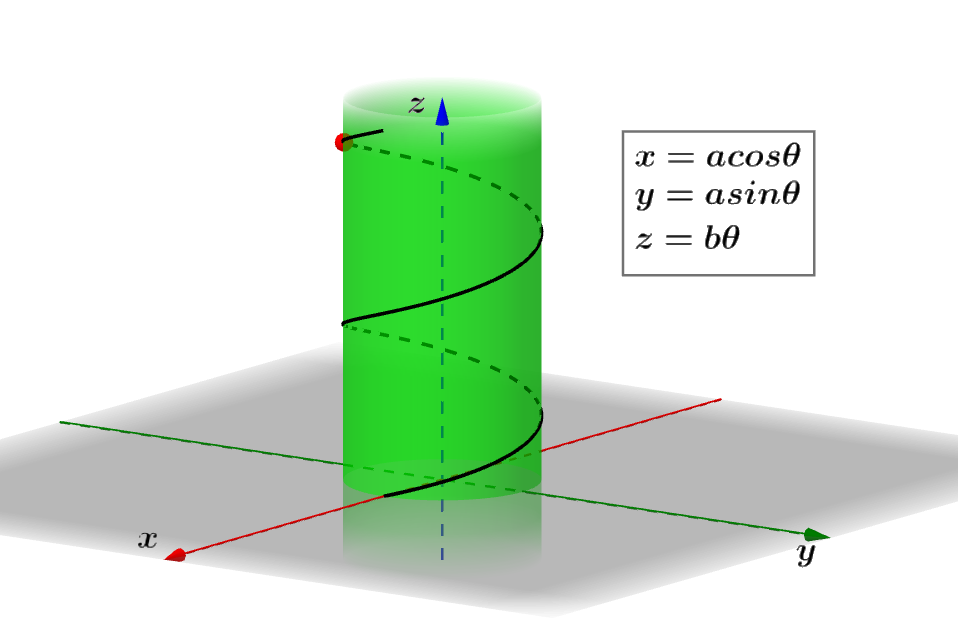
\includegraphics[scale=0.5]{3.png}
	\caption{}
\end{figure}

最直观的例子就是弹簧的螺线,其在不同的地方有相同的疏密,但是不同弹簧疏密不同。假设所有弹簧在水平的投影圆半径相同。此时,几何直观告诉我们,弹簧钢丝绕的越稠密的,其法向量和切向量构成的平面转动越慢,其挠率越小。反之在稀疏的地方,其挠率越大。但其实,这只是一种几何直观,并不完全正确。

简单的证明如下:

设弹簧螺线参数方程为:
$$
\begin{aligned}
    x &= \cos(\theta)      \\
    y &= \sin(\theta)      \\
    z &= k \cdot \theta    \\
\end{aligned}
$$

我们很容易就能将其化为标准绳长参数下的形式:
$$
\begin{aligned}
    x &= \cos(\frac{s}{\sqrt{k^2 + 1}})  \\ 
    y &= \sin(\frac{s}{\sqrt{k^2 + 1}})  \\
    z &= \frac{k \cdot s}{\sqrt{k^2+1}}
\end{aligned}
$$

通过定义计算,我们可以得到
$$
\begin{aligned}
    \vec{T}_x &= -\frac1{\sqrt{k^2 + 1}} \sin(\frac{s}{\sqrt{k^2 + 1}}) \\
    \vec{T}_y &=  \frac1{\sqrt{k^2 + 1}} \cos(\frac{s}{\sqrt{k^2 + 1}}) \\
    \vec{T}_z &= \frac{k}{\sqrt{k^2 + 1}} \\
    \kappa    &= \frac{1}{k^2 + 1} \\
    \vec{N}_x &= -\cos(\frac{s}{\sqrt{k^2 + 1}}) \\
    \vec{N}_y &= -\sin(\frac{s}{\sqrt{k^2 + 1}}) \\
    \vec{N}_z &= 0 \\
    \beta     &= \frac{k}{k^2 + 1}  \\
    \vec{B}_x &=  \frac{k}{\sqrt{k^2 + 1}} \sin(\frac{s}{\sqrt{k^2 + 1}}) \\
    \vec{B}_y &= -\frac{k}{\sqrt{k^2 + 1}} \cos(\frac{s}{\sqrt{k^2 + 1}}) \\
    \vec{B}_z &= \frac{1}{\sqrt{k^2 + 1}}
\end{aligned}
$$

容易看出,挠率只有在 $k \le 1$ 的时候随着 $k$ 减小而单调减(即前文所描述稀疏的地方,其挠率越大),而现实生活中常见的弹簧如果不是过度拉伸,都是绕的比较紧密的,应该有 $k \ll 1$ 。所以在这里理论与几何直观基本符合。

\section{高维曲线}

我们已经用理论推导出了二维和三维曲线的弯曲性质相关的一些参数,也定义了其在二维和三维下的一组标准基。在三维情况下,这组公式被称为 Frenet-Serret 公式 \upcite{ref3}。

我们尝试把这系列公式写成一组更具启发性的形式:

二维:

$$
\frac{d}{ds}
\begin{bmatrix}
    \vec{T} \\
    \vec{N}
\end{bmatrix} = 
\begin{bmatrix}
    0 & \kappa \\
    -\kappa & 0 
\end{bmatrix}
\begin{bmatrix}
    \vec{T}  \\
    \vec{N}
\end{bmatrix}
$$

三维:

$$
\frac{d}{ds}
\begin{bmatrix}
    \vec{T} \\
    \vec{N} \\
    \vec{B}
\end{bmatrix} = 
\begin{bmatrix}
    0 & \kappa & 0\\
    -\kappa & 0 & \beta \\
    0 & -\beta & 0
\end{bmatrix}
\begin{bmatrix}
    \vec{T}  \\
    \vec{N}  \\
    \vec{B} 
\end{bmatrix}
$$

我们因此推测,类似的形式也能推广到更高的维度。

\subsection{高维曲线的高阶曲率}

类似低维的情况,我们依然有定义:

$$
\begin{aligned}
    \vec{T_1} &= \frac{d\vec{r}}{ds} \\ 
\end{aligned}
$$

而利用 $\vec{T}_1\cdot\vec{T}_1 = 1$ 求导,可以定义一个与 $T_1$ 正交的方向 ${\kappa_1} T_2 = \frac{d\vec{T}_1}{ds}$ 。对应二维情况,$T_2$ 就是法向,而 $\kappa_1$ 就是曲率。

再利用 $\vec{T}_2\cdot\vec{T}_2 = 1$ 和 $\vec{T_1}\cdot\vec{T}_2 = 0$ 求导,我们可以得到 $\kappa_1 + \vec{T}_1 \cdot \frac{d\vec{T}_2}{ds} = 0 $ ,其直观涵义就是 $\frac{d\vec{T}_2}{ds}$ 在 $T_1$ 方向的投影为 $-\kappa_1$,因此,我们可以定义第二法向和第二曲率有 $\kappa_2 \vec{T}_3 = \frac{d\vec{T}_2}{ds} + \kappa_1 \vec{T}_1$。对应三维的情况 $T_3$ 就是副法向,而 $\kappa_2$ 就是挠率。

我们猜测,$\forall n \in \mathbb{N}$,有
$$
\begin{aligned}    
    \frac{d\vec{T}_1}{ds}   &= \kappa_1 \vec{T}_2 \\
    \frac{d\vec{T}_2}{ds}   &= -\kappa_1 \vec{T}_1  + \kappa_2 \vec{T}_3 \\
    &...\\
    \frac{d\vec{T}_{n-1}}{ds} &= -\kappa_{n-2} \vec{T}_{n-2}  + \kappa_{n-1} \vec{T}_{n} \\
\end{aligned}
$$

特别的:
$$
\begin{aligned}
    \frac{d\vec{T}_{n}}{ds} &= -\kappa_{n-1} \vec{T}_{n-1}
\end{aligned}
$$

推导过程大致如下:

假设已经推导出对于某个 $j \in [1,n]$,满足下列式子:

$$
\begin{aligned}    
    \frac{d\vec{T}_1}{ds}   &= \kappa_1 \vec{T}_2 \\
    \frac{d\vec{T}_2}{ds}   &= -\kappa_1 \vec{T}_1  + \kappa_2 \vec{T}_3 \\
    ...\\
    \frac{d\vec{T}_{j-1}}{ds} &= -\kappa_{j-2} \vec{T}_{j-2}  + \kappa_{j-1} \vec{T}_{j} \\
\end{aligned}
$$


由正交性,对于 $\forall x,y \in [1,j], x < y$

$$
\vec{T}_x \cdot \vec{T}_y = \delta_{x,y} =
\begin{cases}
    1   ,&\text{if $x = y$}       \\
    0   ,&\text{if $x \ne y$}
\end{cases}
$$

对上式求导,结合已有的式子,可以得出对于 $\forall i < j$ , $\vec{T}_i \cdot \frac{d\vec{T}_j}{ds} +\vec{T}_j \cdot \frac{d\vec{T}_i}{ds} = 0 $。再带入 $\frac{d\vec{T}_i}{ds}$ 的表达式,可以得出:

$$
\vec{T}_i \cdot \frac{d\vec{T}_j}{ds} = 
\begin{cases}
    -\kappa_{j-1},&\text{if $i = j-1$}       \\
    0   ,&\text{if $i \ne j-1$}
\end{cases}
$$ 

因此,我们可以类似将 $\frac{d\vec{T}_j}{ds}$ 写成\textbf{在已有方向的投影}加上\textbf{自己减去这个投影的误差向量}的形式,并且由此得出一个新的方向向量。显然,此时新的方向向量垂直于原有的任何一个方向向量。

$$
\frac{d\vec{T}_{j}}{ds} = -\kappa_{j-1} \vec{T}_{j-1}  + \kappa_{j} \vec{T}_{j+1}
$$

特别地,当 $j = n$的时候,由于维度的限制,并不存在$\vec{T}_{n+1}$,所以此时误差向量就是0,得到

$$
\frac{d\vec{T}_{n}}{ds} = -\kappa_{n-1} \vec{T}_{n-1}
$$

\subsection{小结}

以上便是高维中的高阶法向和高阶曲率的全部内容,我们通过代数的计算,递推得到了一系列标准 $\mathbb{R}^n$ 中的正则曲线的弯曲性质的参数和方向向量。

$$
\begin{aligned}    
    \frac{d\vec{T}_1}{ds}   &= \kappa_1 \vec{T}_2 \\
    \frac{d\vec{T}_2}{ds}   &= -\kappa_1 \vec{T}_1  + \kappa_2 \vec{T}_3 \\
    ...\\
    \frac{d\vec{T}_{n-1}}{ds} &= -\kappa_{n-2} \vec{T}_{n-2}  + \kappa_{n-1} \vec{T}_{n} \\
    \frac{d\vec{T}_{n}}{ds} &= -\kappa_{n-1} \vec{T}_{n-1}
\end{aligned}
$$

或者可以写成更具有启发性的反对称矩阵的形式如下:

$$
\frac{d}{ds}
\begin{bmatrix}
    \vec{T}_1 \\
    \vec{T}_2 \\
    \vec{T}_3 \\
    ...       \\
    \vec{T}_{n-2}\\
    \vec{T}_{n-1}\\
    \vec{T}_{n}
\end{bmatrix} = 
\begin{bmatrix}
        0    &\kappa_1 &    0   &...& 0 & 0 & 0\\
    -\kappa_1&   0     &\kappa_2&...& 0 & 0 & 0\\
    0        &-\kappa_2&   0    &...& 0 & 0 & 0\\
    ...      &   ...   &   ...  &...& ... & ... &  ... \\
    0        &    0    &   0    &...& 0 & \kappa_{n-2} & 0 \\
    0        &    0    &   0    &...&-\kappa_{n-2}& 0  & \kappa_{n-1}\\
    0        &    0    &   0    &...& 0 &-\kappa_{n-1} &  0
\end{bmatrix}
\begin{bmatrix}
    \vec{T}_1 \\
    \vec{T}_2 \\
    \vec{T}_3 \\
    ...       \\
    \vec{T}_{n-2}\\
    \vec{T}_{n-1}\\
    \vec{T}_{n}
\end{bmatrix}
$$


\begin{thebibliography}{30}
    \bibitem{ref1} 维基百科:曲线 \url{https://zh.wikipedia.org/wiki/%E6%9B%B2%E7%BA%BF}
    \bibitem{ref2} 维基百科:曲线的微分几何。 \url{https://zh.wikipedia.org/wiki/%E6%9B%B2%E7%BA%BF%E7%9A%84%E5%BE%AE%E5%88%86%E5%87%A0%E4%BD%95}
    \bibitem{ref3} 维基百科:弗莱纳公式。 \url{https://zh.wikipedia.org/wiki/%E5%BC%97%E8%8E%B1%E7%BA%B3%E5%85%AC%E5%BC%8F}
    \bibitem{ref4} Verstraelen L . Handbook of Differential Geometry, Volume 1[J]. Elsevier, 2000:140–151.

\end{thebibliography}

\end{document}
